\chapter{论文阅读笔记}

\section{Light Gated Recurrent Units for Speech Recogntion}
\href{https://arxiv.org/abs/1803.10225}{Li-GRU}是Mirco Ravanelli于2018年发表的论文,他也是\href{https://arxiv.org/abs/1811.07453}{pytorch-kaldi}的作者。这篇论文主要针对的是对\href{https://arxiv.org/abs/1406.1078}{GRU}(Gated Recurrent Units)的改进,而且Li-GRU是专门为语音识别去设计的。本论文主要的工作有两方面:

(1)去掉了重置门(reset gate),去掉重置门对于模型的效果没什么影响,而且原始的GRU的重置门和更新门之间有冗余,因此去掉重置门的模型结构更合理;
  
(2)将原始GRU中的激活函数Tanh换成了Relu,由于Relu本身函数具备的特性,其效果比Relu要好多。之所以以前的RNN(包括GRU和LSTM)不用Relu,是因为Relu的值可以任意大,RNN不停的迭代中,Relu的值无法控制,容易导致数值不稳定(numerical instability)。本文作者采用了批量正则(Batch Normalization)的方式来避免数值不稳定的情况。这么做既可以避免梯度消失,又可以加速网络收敛,减少网络的时间。


本节的论文笔记分为三个部分:(1)GRU的介绍;(2)Li-GRU的学习;(3)实验配置和结果;(4)个人心得体会。

\subsection{GRU的介绍}
\label{sec:gru}
语音识别是一个序列任务,那么上下文的信息对当前时刻信息的影响很大,RNN的结构表明其可以动态的决定对于当前时间步使用多少上下文的信息。但是RNN存在的梯度消失和爆炸问题使得其学习长期依赖变得困难。所以一般我们都会使用一种门控RNN(Gated RNN)来解决这个问题。门控RNN的核心思想是引入一种门机制来控制不同时间步之间的信息流动。

常用的门控RNN有两种:LSTM和GRU。LSTM的结构复杂且运算效率比较低,LSTM有三个门,而GRU只有两个,所以运算起来快很多。而本论文也是基于GRU做的改进,所以不讨论LSTM。

GRU的计算公式如下:
\begin{align}
z_t &= \sigma(W_{z}x_{t}+U_{z}h_{t-1}+b_z) \label{eqn:up-gate} \\
r_t &= \sigma(W_{r}x_{t}+U_{r}h_{t-1}+b_r) \label{eqn:re-gate} \\
\tilde{h}_{t} &= tanh(W_{h}x_{t}+U_{h}(h_{t-1}\odot{r_{t}})+b_{h}) \label{eqn:candi-h} \\
h_{t} &= z_{t}\odot{h_{t-1}} + (1-z_{t})\odot\tidle{h}_{t}  \label{eqn:final-h}
\end{align}
其中
\begin{itemize}
  \item \textit{$x_t$:t时刻输入特征向量} 
  \item \textit{$r_t$:t时刻重置门向量}  
  \item \textit{$u_t$:t时刻更新门向量}
  \item \textit{$h_t$:t时刻状态向量}
  \item \textit{$\tidle{h}_t$:t时刻候选状态向量}
  \item \textit{$W,U,b$:参数矩阵和向量}

\end{itemize}\\


由公式\ref{eqn:final-h}可知,当前状态向量$h_t$是前一刻状态向量$h_{t-1}$和当前时刻的状态候选向量$\tilde{h}_{t}$之间的一个\href{https://zh.wikipedia.org/zh-hans/\%E7\%BA\%BF\%E6\%80\%A7\%E6\%8F\%92\%E5\%80\%BC}{线性插值}。两者之间的权重由更新门$z_{t}$决定,权重的值表示了更新信息的多少。这个线性插值就是GRU学习长期依赖的核心。如果$z_{t}$接近于$1$,那么先前状态的信息就得以保留,以此学习到间隔长的时间步之间的信息关联。如果$z_t$接近于$0$,那么网络更倾向于候选状态$\tilde{h}_{t}$,而候选状态更依赖于当前输入和临近时间步的状态。同时候选状态还依赖于重置门$r_{t}$,其使得模型通过忘记之前计算的状态来清除过去的记忆。

GRU的模型结构图如\ref{fig:gru}所示。
\begin{figure}[htbp]
  \centering
  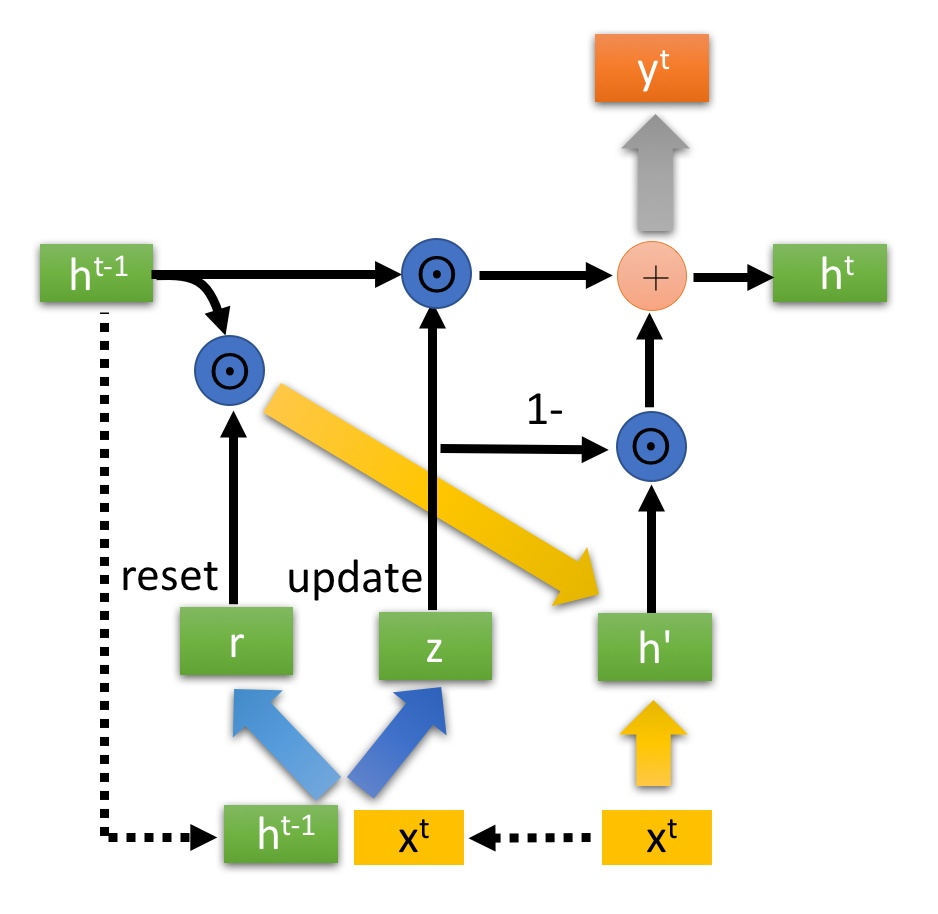
\includegraphics[width=0.45\textwidth]{gru-architecture}
  \caption{GRU模型结构图 \label{fig:gru}}
\end{figure}

\subsection{Li-GRU的学习}
\label{sec:li-gru}
本论文对GRU的改进主要涉及到三个部分:重置门、ReLU激活函数和BN。

1.移除重置门:

对于序列中可能出现的 significant discontinuity,重置门可以起到一个清除过去信息的作用。比如说语言建模,当输入从一个句子跳转到另一个语义无关的句子的时候,重置门就可以起到很好的作用:避免过去无关信息对当前状态的干扰。但是对于语音识别来说,重置门的作用可能就不明显了,语音识别中的输入变化都比较小(一般的偏移量才10ms),这表明过去的信息还是挺有用的。即便是元音(Vowel)和擦音(Fricative)间的边界有很强的不连续现象,完全去掉过去信息也可能是有害的。另外基于一些音素的转移更相似,存住 phonotactic features 还是很有用的。

与此同时,重置门和更新门之间存在着某种冗余。也就是说$z_t$和$r_t$的变化比较同步,当前输入信息比较重要的时候,$z_t$和$r_t$都比较小;过去时刻信息比较重要的时候,$z_t$和$r_t$都比较大。拿TIMIT中的一段音频来看,更新门和重置门的平均激活值有着时域上的关联性,如图\ref{fig:ru-correlation}。
\begin{figure}[htbp]
  \centering
  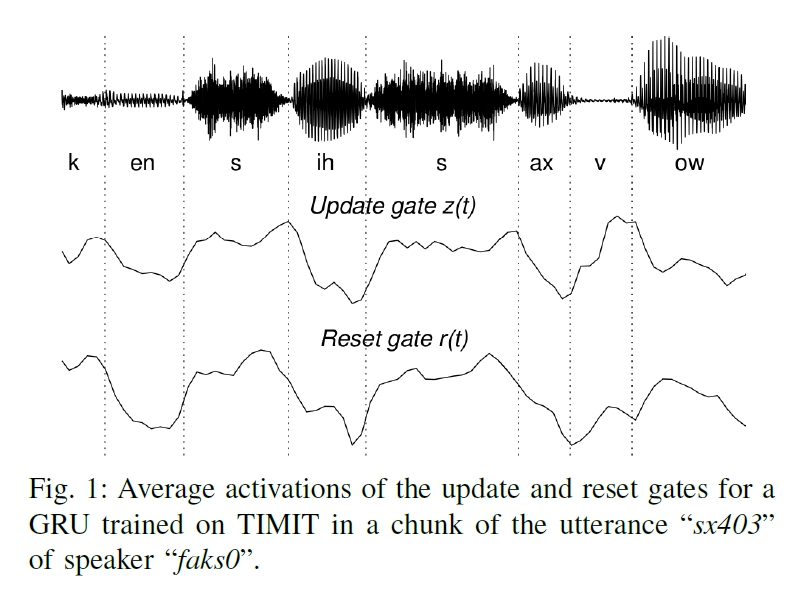
\includegraphics[width=0.45\textwidth]{rucor}
  \caption{TIMIT中更新门与重置门音频上的时域关联 \label{fig:ru-correlation}}
\end{figure}

两个门之间的冗余程度可以量化描述,其公式 cross-correlation $C(z,r)$如下:
\begin{align}
\label{eqn:rucor}
C(z,r) = \bar{z}_t \star \bar{r}_t
\end{align}
其中:
\begin{itemize}
  \item \textit{$\bar{z}_t$:更新门神经元的平均激活值}
  \item \textit{$\bar{r}_t$:重置门神经元的平均激活值}
  \item \textit{$\star$:cross-correlation 的算子} 
\end{itemize}

图\ref{fig:aver-cor}显示了重置门和更新门的 cross-correlation。门激活值计算的是所有的输入帧,所有的隐藏神经元的激活值计算了个平均。从图中我们可以看到重置门和更新门之间相似度还挺高,因此冗余程度也很高。
\begin{figure}[htbp]
  \centering
  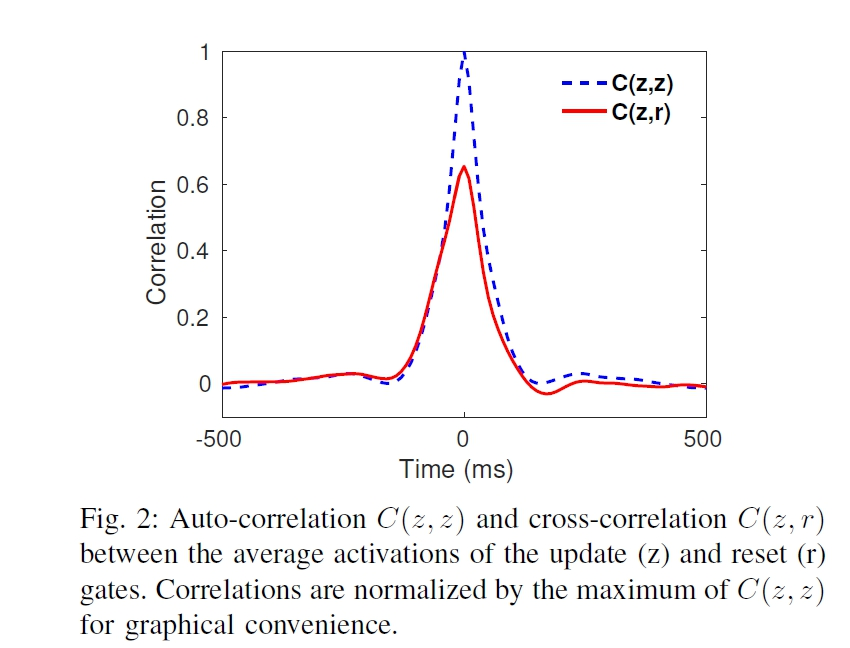
\includegraphics[width=0.45\textwidth]{aver-cor}
  \caption{Auto-correlation $C(z,z)$和cross-correlation $C(z,r)$ \label{fig:aver-cor}}
\end{figure}

因此我们决定去掉重置门,那么公式\ref{eqn:candi-h}就变成了公式\ref{eqn:candi-h-no-reset}。这么处理之后,运算效率就提高了,就剩下一个门,所以GRU的结构变得更紧凑了。
\begin{align}
\label{eqn:candi-h-no-reset}
\tilde{h}_{t} &= tanh(W_{h}x_{t}+U_{h}h_{t-1}+b_{h})
\end{align}

2. ReLU激活函数

我们将tanh替换成ReLU。tanh其实在前馈神经网络中很少使用,因为当神经网络的层数变深时,它就容易陷入左右的边界值$-1$和$1$,此时的梯度接近于$0$,网络参数更新缓慢,收敛的也就很慢。ReLU就不存在这样的问题,但是ReLu的值域没有边界,因此容易出现一些数值问题,为了解决这个问题,我们将ReLU和BN一起使用,这样就很不存在数值问题了。将tanh改为ReLU之后,GRU的公式如下:
\begin{align}
\label{eqn:candi-h-no-reset-relu}
\tilde{h}_{t} &= ReLU(W_{h}x_{t}+U_{h}h_{t-1}+b_{h})
\end{align}

3.BN

神经网络训练时,计算每一个 mini-batch 每层激活前输出的均值和方差,再利用均值和方差对激活前输出进行归一化能够解决所谓的 internal covariate shift 问题,这个就是传说中的Batch Normalization。BN既可以加快网络训练速度,又可以提高模型的效果。本文中只对前馈部分进行BN操作,因为其只对前馈神经网络进行操作,完全可以实现并行计算。其公式如下:
\begin{align}
z_t &= \sigma(BN(W_{z}x_{t})+U_{z}h_{t-1}) \label{eqn:bn-up-gate} \\
\tilde{h}_{t} &= ReLU(BN(W_{h}x_{t})+U_{h}h_{t-1}) \label{bn-eqn:candi-h} \\
h_{t} &= z_{t}\odot{h_{t-1}} + (1-z_{t})\odot\tidle{h}_{t}  \label{eqn:bn-final-h}
\end{align}
其中$BN(\cdot)$如公式\ref{eqn:bn}所示,$\mu_{b}$和$\sigma_{b}$分别为当前mini-batch的均值和方差。
\begin{align}
\label{eqn:bn}
BN(a) = \gamma \odot \frac{a-\mu_{b}}{\sqrt{(\sigma_b)^{2}+\epsilon}} + \beta
\end{align}

因为BN中已经包含了$\beta$,因此之前公式中的偏置$b_z$和$b_h$就不再需要了。Li-GRU将ReLU和BN结合起来,既利用了ReLU和BN两者的优点,同时还避免了ReLU的数值不稳定问题。

\subsection{个人心得体会}
\label{sec:ligru-pers}
综上所言,Li-GRU通过减少了一个重置门来达到轻量级的效果,与此同时根据语音识别任务的特殊性,其认为语音序列任务中,对过往记忆清零对模型效果是有伤害的,而且重置门和更新门之间关联比较深,两个门显得冗余,因此其去掉了重置门。为了让网络更新更快,效果更好,以Relu函数代替了tanh作为候选状态的激活函数,同时以BN来解决Relu无边界的数值问题。BN还可以帮助快速训练和提升效果。

附上一些音素的分类,如表\ref{tab:phone-category}
\begin{table}[htbp]
   \centering
   \caption{音素分类及示例}
     \begin{tabular*}{1\textwidth}{@{\extracolsep{\fill}}ccc}
     \toprule
     Phonetic Cat. &音素类别       & Phone Lists \\
     \midrule
     Vowels        &元音          & \{iy, ih, eh, ae, ..., oy, aw, ow, er\}  \\
     Liquids       &流音          & \{l, r, y, w, el\}  \\
     Nasals        &鼻音          & \{en, m, n, ng\}  \\
     Fricatives    &擦音          & \{ch, jh, dh, z, v, f, th, s, sh, hh, ,zh\}   \\
     Stops         &塞音          & \{b, d, g, p, t, k, dx, cl, vcl, epi\}   \\
     \bottomrule
     \end{tabular}%
   \label{tab:phone-category}%
 \end{table}%

